\chapter{Pengantar Optimasi dan Komputasi Evolusioner}

  Algoritma genetika (GA) adalah metode pencarian berbasis populasi yang terinspirasi dari seleksi alam dan genetika. Mereka mempertahankan populasi solusi kandidat yang dikodekan sebagai string, secara iteratif menghasilkan generasi baru dengan memilih individu terbaik, menggabungkan informasi mereka, dan terkadang memperkenalkan variasi acak. Meskipun stokastik dalam operatornya, GA bukan random walk buta: mereka mempertahankan dan mengeksploitasi informasi historis tentang solusi yang baik untuk menghasilkan titik pencarian baru yang menjanjikan dan dengan demikian mendorong eksplorasi dan eksploitasi ruang kompleks yang efisien.

  Keluarga metode ini dikembangkan dari karya fundamental Holland dan rekan-rekannya untuk memodelkan proses adaptif yang diamati di alam dan merancang sistem buatan yang mewujudkan mekanisme tersebut. Tujuan utamanya adalah ketahanan—kemampuan untuk menyeimbangkan efisiensi dengan keandalan di berbagai lingkungan masalah—yang membuat GA menarik ketika biaya perancangan ulang tinggi atau ketika struktur masalah melanggar asumsi umum (misalnya, kontinuitas, diferensiabilitas, atau unimodalitas). Karena mereka secara konseptual sederhana, dapat diterapkan secara luas, dan efektif secara empiris dalam optimasi dan kontrol, algoritma genetika telah menjadi alat praktis di berbagai domain teknik, sains, dan bisnis \cite{goldberg1989genetic}.

  Untuk menempatkan algoritma genetika dalam konteks, pertama-tama kami memberikan definisi ringkas tentang optimasi — kelas masalah yang biasanya diselesaikan menggunakan GA.
    Kami mendefinisikan optimasi sebagai proses menemukan solusi terbaik dari sekumpulan alternatif yang tersedia. Dalam istilah matematis, masalah optimasi dapat diformulasikan sebagai:

  \begin{equation}
  \begin{aligned}
  \text{minimumkan (atau maksimumkan)} \quad & f(x) \\
  \text{dengan batasan} \quad & g_i(x) \leq 0, \quad i = 1, 2, \ldots, m \\
  & h_j(x) = 0, \quad j = 1, 2, \ldots, p \\
  & x \in X
  \end{aligned}
  \end{equation}

  di mana:
  \begin{itemize}
      \item $f(x)$ adalah fungsi objektif yang akan dioptimasi
      \item $g_i(x)$ adalah batasan ketidaksetaraan
      \item $h_j(x)$ adalah batasan persamaan
      \item $X$ adalah wilayah yang layak
  \end{itemize}

    Masalah optimasi berbeda berdasarkan jenis variabel (diskrit, kontinu, atau mixed-integer) dan berdasarkan properti struktural seperti linearitas, konveksitas, dan jumlah objektif. 
    Metode solusi tradisional mencakup teknik berbasis gradien (misalnya, metode Newton dan quasi-Newton) untuk masalah kontinu halus, pemrograman linear (metode Simplex dan interior-point) untuk model linear, dan metode diskrit (branch-and-bound, pemrograman dinamis) untuk masalah kombinatorial. 
    Namun, metode tradisional ini memiliki keterbatasan ketika diterapkan pada banyak masalah dunia nyata yang kompleks. Dalam bagian berikut kami menyoroti tiga tantangan utama di mana pendekatan konvensional sering mengalami kesulitan, dan menjelaskan bagaimana algoritma genetika dapat membantu mengatasinya.


    Masalah pertama dengan metode optimasi tradisional adalah kecenderungan mereka untuk terjebak dalam optimum lokal.
    Dalam lanskap multi-modal dengan banyak puncak dan lembah, pencarian berbasis gradien dapat konvergen ke 
    optimum lokal daripada optimum global. Ini terjadi karena metode-metode ini bergantung pada informasi gradien lokal untuk memandu proses pencarian. Ketika pencarian mencapai optimum lokal, gradien 
    menjadi nol, menyebabkan algoritma berhenti berkembang. Keterbatasan ini terutama 
    bermasalah dalam ruang berdimensi tinggi di mana jumlah optimum lokal dapat tumbuh secara eksponensial.

  \begin{figure}[H]
    \centering
    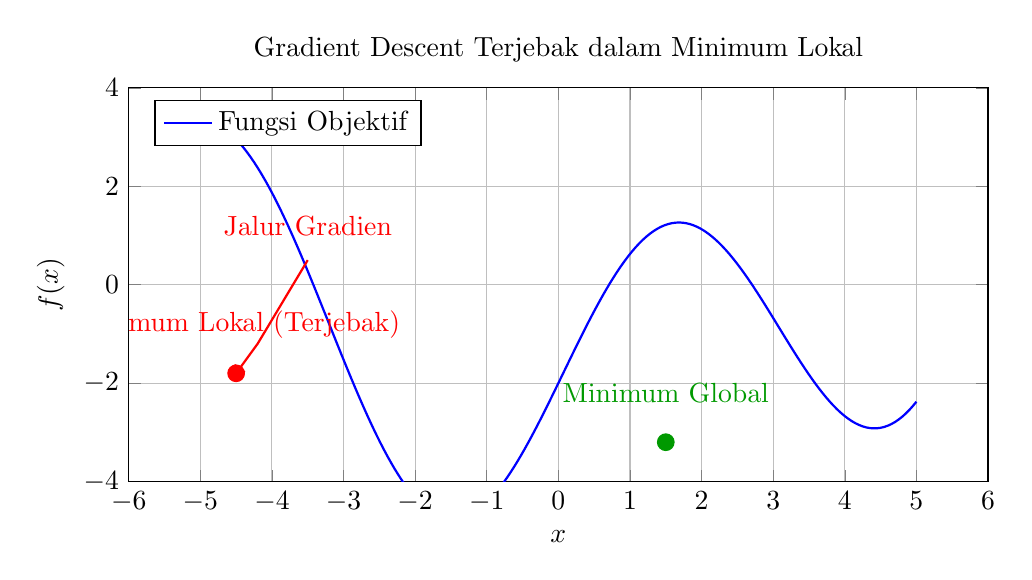
\begin{tikzpicture}
    \begin{axis}[
      width=0.9\textwidth,
      height=5cm,
      scale only axis,
      ymin=-4,
      ymax=4,
      xlabel={$x$},
      ylabel={$f(x)$},
      title={Gradient Descent Terjebak dalam Minimum Lokal},
      grid=major,
      legend pos=north west,
    ]
    % Fungsi multi-modal
    \addplot[blue, thick, domain=-5:5, samples=200] {sin(deg(x))*3 + 0.1*x^2 - 2};
    \addlegendentry{Fungsi Objektif}

    % Titik minimum lokal
    \addplot[red, mark=*, mark size=3pt] coordinates {(-4.5, -1.8)};
    \node[red] at (axis cs:-4.5,-0.8) {Minimum Lokal (Terjebak)};

    % Titik minimum global
    \addplot[green!60!black, mark=*, mark size=3pt] coordinates {(1.5, -3.2)};
    \node[green!60!black] at (axis cs:1.5,-2.2) {Minimum Global};

    % Jalur gradient descent
    \addplot[red, thick, ->] coordinates {(-3.5, 0.5) (-4.2, -1.2) (-4.5, -1.8)};
    \node[red] at (axis cs:-3.5,1.2) {Jalur Gradien};
    \end{axis}
    \end{tikzpicture}
    \caption{Metode berbasis gradien tradisional mengikuti gradien lokal dan menjadi terjebak dalam optimum lokal, tidak mampu melarikan diri untuk menemukan optimum global.}
  \end{figure}

  Masalah kedua dengan metode berbasis gradien adalah bahwa mereka memerlukan fungsi objektif yang dapat didiferensiasikan. Ini menjadi keterbatasan signifikan ketika menangani masalah dunia nyata yang melibatkan diskontinuitas, sudut tajam, atau lompatan diskrit.
  Masalah seperti itu umum dalam desain teknik, penjadwalan, dan optimasi kombinatorial.

  \begin{figure}[H]
  \centering
  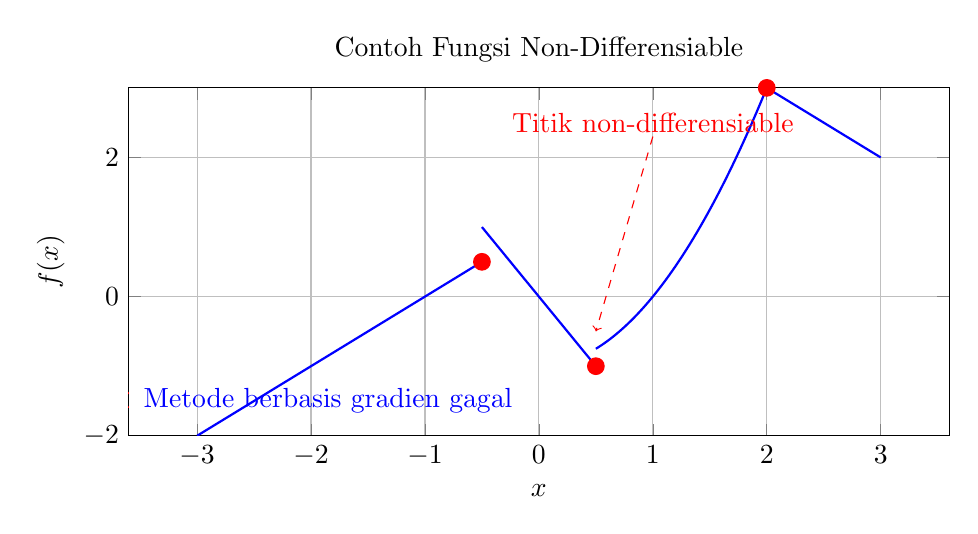
\begin{tikzpicture}
  \begin{axis}[
      width=12cm,
      height=6cm,
      xlabel={$x$},
      ylabel={$f(x)$},
      title={Contoh Fungsi Non-Differensiable},
      grid=major,
      ymin=-2,
      ymax=3,
  ]
  % Fungsi piecewise dengan diskontinuitas
  \addplot[blue, thick, domain=-3:-0.5, samples=50] {x + 1};
  \addplot[blue, thick, domain=-0.5:0.5, samples=50] {-2*x};
  \addplot[blue, thick, domain=0.5:2, samples=50] {x^2 - 1};
  \addplot[blue, thick, domain=2:3, samples=50] {-x + 5};

  % Menandai diskontinuitas
  \addplot[red, mark=*, mark size=3pt, only marks] coordinates {(-0.5, 0.5) (0.5, -1) (2, 3)};
  \node[red] at (axis cs:1, 2.5) {Titik non-differensiable};
  \draw[red, dashed, ->] (axis cs:1, 2.3) -- (axis cs:0.5, -0.5);

  \node[blue] at (axis cs:-2, -1.5) {\textcolor{red}{\textbf{×}} Metode berbasis gradien gagal};
  \end{axis}
  \end{tikzpicture}
  \caption{Fungsi dengan diskontinuitas, sudut tajam, atau lompatan diskrit tidak dapat dioptimalkan menggunakan metode berbasis gradien.}
  \end{figure}


    Sementara metode diskrit seperti pemrograman dinamis dapat menangani diskontinuitas dan struktur kombinatorial, baik algoritma berbasis gradien maupun algoritma diskrit eksak mengalami kutukan dimensionalitas: komputasi biasanya menjadi tidak dapat dilacak seiring dimensi masalah tumbuh.

  \begin{figure}[H]
  \centering
  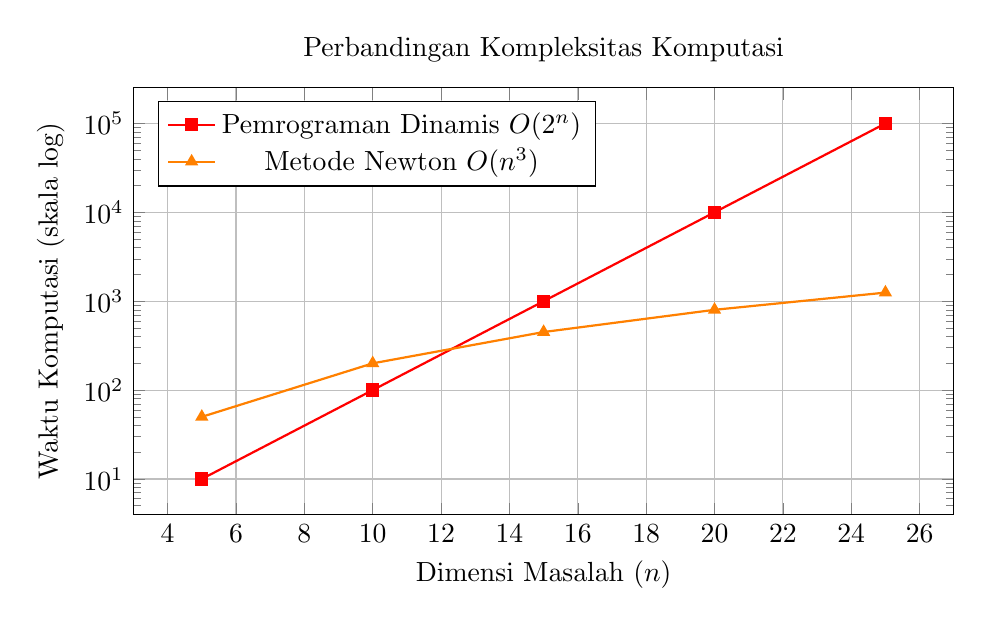
\begin{tikzpicture}
  \begin{axis}[
      width=12cm,
      height=7cm,
      xlabel={Dimensi Masalah ($n$)},
      ylabel={Waktu Komputasi (skala log)},
      title={Perbandingan Kompleksitas Komputasi},
      ymode=log,
      legend pos=north west,
      grid=major,
  ]
  % Pertumbuhan eksponensial untuk metode tradisional
  \addplot[red, thick, mark=square*] coordinates {
      (5, 10)
      (10, 100)
      (15, 1000)
      (20, 10000)
      (25, 100000)
  };
  \addlegendentry{Pemrograman Dinamis $O(2^n)$}

  % Pertumbuhan polinomial untuk Newton
  \addplot[orange, thick, mark=triangle*] coordinates {
      (5, 50)
      (10, 200)
      (15, 450)
      (20, 800)
      (25, 1250)
  };
  \addlegendentry{Metode Newton $O(n^3)$}

  \end{axis}
  \end{tikzpicture}
    \caption{Metode optimasi tradisional sering menunjukkan pertumbuhan eksponensial atau polinomial tinggi dalam waktu komputasi seiring dimensi masalah meningkat, membuat mereka tidak praktis untuk masalah skala besar.}
  \end{figure}


    Oleh karena itu, kita dapat merangkum bagaimana algoritma genetika secara efektif mengatasi keterbatasan fundamental metode optimasi tradisional dalam tabel berikut:
  \begin{figure}[H]
  \centering
  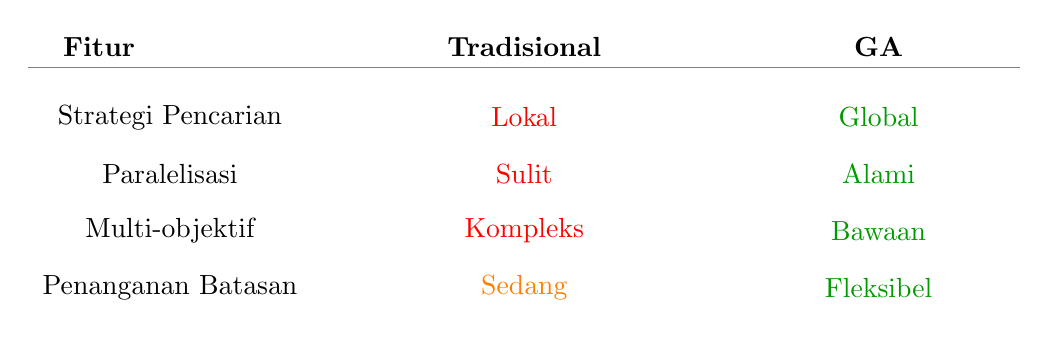
\begin{tikzpicture}[scale=0.9]
      % Baris perbandingan
      \node[font=\bfseries] at (1, 4) {Fitur};
      \node[font=\bfseries] at (7, 4) {Tradisional};
      \node[font=\bfseries] at (12, 4) {GA};
      
      \draw[gray] (0, 3.7) -- (14, 3.7);
      
      \node[align=left] at (2, 3) {Strategi Pencarian};
      \node[red] at (7, 3) {Lokal};
      \node[green!60!black] at (12, 3) {Global};
      
      \node[align=left] at (2, 2.2) {Paralelisasi};
      \node[red] at (7, 2.2) {Sulit};
      \node[green!60!black] at (12, 2.2) {Alami};
      
      \node[align=left] at (2, 1.4) {Multi-objektif};
      \node[red] at (7, 1.4) {Kompleks};
      \node[green!60!black] at (12, 1.4) {Bawaan};
      
      \node[align=left] at (2, 0.6) {Penanganan Batasan};
      \node[orange] at (7, 0.6) {Sedang};
      \node[green!60!black] at (12, 0.6) {Fleksibel};
  \end{tikzpicture}
  \caption{Perbandingan komprehensif menunjukkan bagaimana GA mengatasi keterbatasan fundamental metode optimasi tradisional.}
  \end{figure}

  \section{Pengantar Komputasi Evolusioner}
  Komputasi evolusioner adalah keluarga algoritma pencarian stokastik berbasis populasi yang terinspirasi oleh prinsip-prinsip evolusi biologis~\cite{holland1975adaptation, eiben2015introduction}. Anggota keluarga ini beroperasi pada populasi solusi kandidat dan berulang kali menerapkan seleksi (prinsip survival of the fittest), rekombinasi atau crossover (untuk bertukar informasi antar solusi), dan mutasi (untuk memperkenalkan variasi baru). Mekanisme ini memungkinkan algoritma evolusioner untuk mempertahankan dan menggabungkan kembali komponen solusi yang berguna sambil terus mengeksplorasi wilayah baru dari ruang pencarian.

  Properti ini memberikan pendekatan evolusioner sejumlah keuntungan praktis untuk masalah optimasi yang sulit. Karena mereka bebas turunan dan hanya memerlukan evaluasi fungsi, metode evolusioner secara alami cocok untuk masalah optimasi black-box, termasuk fungsi objektif yang diskontinu, bising, tidak dapat didiferensiasikan, atau mengalami lompatan diskrit. Pencarian berbasis populasi mereka memberikan ketahanan terhadap optimum lokal dan memungkinkan evaluasi paralel kandidat solusi secara langsung, yang berharga untuk evaluasi fitness yang mahal. Sementara algoritma evolusioner umumnya tidak memberikan jaminan optimalitas formal, dengan representasi dan operator yang tepat mereka menawarkan kinerja heuristik yang andal di berbagai domain variabel kontinu, diskrit, dan campuran.

  Bidang komputasi evolusioner mencakup beberapa keluarga yang mapan, masing-masing menekankan pilihan desain yang berbeda. Algoritma Genetika (GA) adalah salah satu formulasi paling awal dan paling berpengaruh, menekankan pengkodean panjang tetap dan operator crossover dan mutasi yang terinspirasi secara biologis~\cite{holland1975adaptation, goldberg1989genetic}. Strategi Evolusi (ES) berkonsentrasi pada strategi mutasi yang dapat beradaptasi sendiri dan sangat efektif untuk optimasi kontinu bernilai nyata~\cite{back1996evolutionary}. Pemrograman Evolusioner (EP) secara historis fokus pada evolusi model perilaku dan skema mutasi stokastik daripada rekombinasi eksplisit~\cite{fogel1995evolutionary, fogel2006evolutionary}. Pemrograman Genetika (GP) memperluas kerangka kerja ke struktur panjang variabel seperti program komputer dan pohon ekspresi, memungkinkan sintesis program otomatis~\cite{koza1992genetic}.

  Algoritma evolusioner telah berhasil diterapkan di berbagai bidang teknik, sains, dan bisnis. Dalam desain teknik mereka digunakan untuk mengoptimalkan konfigurasi sistem kompleks di mana evaluasi objektif mungkin mahal atau tidak dapat didiferensiasikan~\cite{yildiz2023novel}. Dalam pembelajaran mesin, metode evolusioner telah digunakan baik untuk mengembangkan arsitektur jaringan saraf dan untuk mengoptimalkan bobot ketika informasi gradien tidak tersedia atau tidak dapat diandalkan~\cite{montana1989training, murad2025hybrid}. Penjadwalan, pembuatan jadwal waktu, perutean (termasuk Travelling Salesman Problem), dan masalah kombinatorial lainnya adalah aplikasi alami karena pengkodean yang fleksibel dan operator rekombinasi khusus yang menghormati struktur masalah~\cite{gu2022hybrid, fajrin2020multi}. Di luar domain ini, komputasi evolusioner telah menemukan peran dalam bioinformatika, pemodelan keuangan, dan desain strategi permainan otomatis, menunjukkan utilitas praktis yang luas~\cite{gen2007genetic, sivanandam2008introduction, eiben2015introduction}.

  Untuk membuat ide-ide ini konkret, pertimbangkan dua contoh ringkas yang biasa digunakan untuk ilustrasi pedagogis. Masalah mainan sederhana adalah memaksimalkan fungsi kuadrat $f(x)=x^2$ pada domain diskrit $0\leq x\leq31$. Dengan pengkodean biner (kromosom 5-bit), siklus berulang seleksi, crossover, dan mutasi mengkonsentrasikan blok bangunan yang mewakili nilai $x$ yang lebih tinggi sampai, biasanya dalam beberapa generasi, individu yang mengkodekan optimum ($x=31$) mendominasi populasi. Contoh ini menyoroti bagaimana rekombinasi mengakumulasi solusi parsial yang berguna (blok bangunan) bahkan ketika populasi awal acak.

  Dalam contoh kombinatorial yang lebih menantang, Travelling Salesman Problem (TSP) meminta tur terpendek yang mengunjungi sekumpulan kota. Algoritma Genetika untuk TSP menggunakan representasi dan operator crossover yang mempertahankan properti urutan kota (misalnya, crossover berbasis urutan atau posisi) dan operator mutasi yang melakukan gangguan lokal tur. Sementara GA tidak menjamin optimalitas untuk masalah NP-hard seperti TSP, mereka sering menghasilkan solusi perkiraan berkualitas tinggi dengan cepat dan dapat dikombinasikan dengan pencarian lokal (pendekatan hibrid) untuk peningkatan lebih lanjut.

  \begin{figure}[h]
  \centering
  \includegraphics[width=0.7\textwidth]{figures/buku_ajar_page_4.png}
  \caption{Ilustrasi siklus GA dan variasinya}
  \label{fig:ga_intro_cycle}
  \end{figure}


  Meskipun Algoritma Genetika Generasi Sederhana berfungsi sebagai kerangka dasar, berbagai modifikasi telah dikembangkan untuk meningkatkan kinerja dalam menangani kompleksitas masalah. Beberapa modifikasi ini termasuk varian yang telah dipelajari dengan baik berikut.

  Algoritma Genetika Hibrid menggabungkan pencarian evolusioner global dengan prosedur peningkatan lokal yang ditargetkan untuk mengeksploitasi kekuatan komplementer dari kedua paradigma. Desain hibrid tipikal menggunakan GA untuk eksplorasi luas sambil menerapkan pencarian lokal deterministik atau stokastik (misalnya, hill-climbing, pencarian tabu, atau heuristik khusus masalah) untuk menyempurnakan individu terpilih atau solusi terbaik yang ditemukan sejauh ini. Dengan menggabungkan diversifikasi dan intensifikasi, metode hibrid sering mencapai konvergensi lebih cepat dan hasil berkualitas lebih tinggi pada tugas optimasi praktis~\cite{majhi2025novel, murad2025hybrid}.

  Algoritma Genetika Adaptif memodifikasi parameter kontrol secara online menggunakan umpan balik dari statistik populasi seperti tingkat peningkatan fitness, keberhasilan operator, atau ukuran keragaman genetik. Adaptasi dapat diimplementasikan secara eksternal melalui aturan kontrol atau secara internal dengan mengkodekan parameter dalam individu sehingga evolusi itu sendiri memilih pengaturan yang efektif. Mekanisme ini mengurangi penyetelan manual dan membantu mempertahankan keseimbangan eksplorasi-eksploitasi yang produktif di berbagai fase pencarian~\cite{shams2025resolving, srinivas1994genetic}.

  Algoritma Genetika Paralel mengeksploitasi perangkat keras paralel modern dengan mendistribusikan komputasi dan/atau struktur populasi. Model berbutir kasar (pulau) memegang sub-populasi pada prosesor yang berbeda dengan migrasi sesekali untuk berbagi informasi; model berbutir halus atau master-slave memparalelkan evaluasi fitness untuk mengurangi waktu wall-clock. Paralelisme tidak hanya mempercepat komputasi tetapi juga dapat meningkatkan ketahanan pencarian dengan melestarikan banyak relung dan mengurangi konvergensi prematur~\cite{eiben2015introduction}.
    \section{Variasi Algoritma Genetika}

    Meskipun Algoritma Genetika generasi sederhana berfungsi sebagai kerangka dasar, berbagai modifikasi telah dikembangkan untuk meningkatkan kinerja pada masalah kompleks. Variasi umum meliputi:

    \subsection{Tinjauan}
    \begin{itemize}
        \item \textbf{GA Hibrid:} Menggabungkan Algoritma Genetika dengan pencarian lokal atau metode optimasi lain untuk menyempurnakan solusi yang menjanjikan setelah eksplorasi global~\cite{majhi2025novel, murad2025hybrid}.
        \item \textbf{GA Adaptif:} Secara dinamis menyesuaikan parameter seperti probabilitas crossover dan mutasi berdasarkan umpan balik populasi untuk menyeimbangkan eksplorasi dan eksploitasi~\cite{shams2025resolving, srinivas1994genetic}.
        \item \textbf{GA Paralel:} Membagi populasi menjadi sub-populasi di seluruh prosesor (model pulau, master-slave, dll.) dan secara berkala bertukar individu untuk mempercepat pencarian dan mempertahankan keragaman.
    \end{itemize}


  \section{Bacaan Lebih Lanjut}
  \begin{itemize}
      \item Deb, K. (2001). Multi-objective optimization using evolutionary algorithms.
      \item Eiben, A. E., \& Smith, J. E. (2015). Introduction to evolutionary computing.
      \item Goldberg, D. E. (1989). Genetic algorithms in search, optimization, and machine learning.
  \end{itemize}